
%\usepackage{graphicx}
%\usepackage{subfigure}
%\usepackage{amsmath,amssymb}
%\usepackage[english]{babel}
%\usepackage[utf8]{inputenc}
%\usepackage[ruled,vlined]{algorithm2e}
%\usepackage{url}
%\usepackage{float}
%\usepackage{multirow} 
%\usepackage{booktabs}
%\usepackage[disable]{todonotes}
%\usepackage{todonotes}
%\usepackage{booktabs}
%\usepackage{mdframed}
%\usepackage{wrapfig}
%\usepackage{caption}
%\usepackage{tikz}
%\usepackage{verbatim}
%\usepackage{afterpage}
%\usepackage[active,tightpage]{preview}
%\PreviewEnvironment{tikzpicture}
%\setlength\PreviewBorder{5pt}%

%\usepackage{siunitx}%number formatting inside tables
\sisetup{
round-mode = places,
detect-family = true,
detect-inline-family = math,
detect-weight=true,
detect-inline-weight = math
}%

%\begin{document}


\chapter{Cross-Document Co-reference Resolution using Latent Features}


%\author{
%Axel-Cyrille Ngonga Ngomo$^{\diamondsuit}$ \and
%Michael R\"oder$^{\spadesuit\diamondsuit}$ \and 
%Ricardo Usbeck$^{\spadesuit\diamondsuit}$ 
%\institute{
%${\diamondsuit}$ University of Leipzig, Germany, 
%${\spadesuit}$ R\,\&\,D, Unister~GmbH, Leipzig, Germany, 
%\newline email: \{ngonga$|$usbeck\}@informatik.uni-leipzig.de
%}
%}

%\maketitle

%\newmdtheoremenv{ex}{Example}
\newcommand{\goodgap}{%
%\hspace{\subfigtopskip}%
%\hspace{\subfigbottomskip}
}
\todo[inline]{adjust goodgap}
%\begin{abstract}
Over the last years, entity detection approaches which combine named entity recognition and entity linking have been used to detect mentions of RDF resources from a given reference knowledge base in unstructured data. In this paper, we address the problem of assigning a single URI to named entities which stand for the same real-object across documents but are not yet available in the reference knowledge base. This task is known as cross-document co-reference resolution and has been addressed by manifold approaches in the past. We present a preliminary study of a novel take on the task based on the use of latent features derived from matrix factorizations combined with parameter-free graph clustering. 
%We study whether this approach achieves better results than the simple approaches used in most tools so far by measuring the accuracy of the clusters we detect on several benchmark datasets.
We study the influence of different parameters (window size, rank, hardening) on our approach by comparing the F-measures we achieve on the $\mbox{N}^3$ benchmark.
Our results suggest that using latent features leads to higher F-measures with an increase of up to 20.5\% on datasets of the $\mbox{N}^3$ collection.
%\end{abstract} 

%\todo[inline]{Full paper with a maximum of 12 pages including references
%Short paper with a maximum of 6 pages including references}

\section{Introduction}
%\todo[inline]{Removed: The abstact contains "deterministic matrix factorization algorithm". But is it still deterministic?}
%\todo[inline]{Axel}
The Document Web contains a large amount of information that is still not available on the Web of Data.
For example, open extraction frameworks for unstructured data have been shown to harvest a considerable amount of new triples pertaining to real-objects for which no URI is available~\cite{GER+13}.
While no URI has been assigned to the said real-world objects, facts pertaining to these objects can be distributed across manifold data sources.
Hence, simple URI generation approaches based on the labels of named entities can easily fail to generate the same URI when relying on two different labels that stand for the same real-world object.
For example, simple URI generation schemes based on strings would fail to generate the same URI when presented with the strings ``P. Diddy'' and ``Puff Daddy'' as labels for resources.
Moreover, they would generate the same URI for ``Golf'' across different documents even if the ``Golf'' stood for the sport in some documents and for the car in others.
In literature, detecting that two labels stand for the same real-object even across documents is referred to as \emph{cross-document co-reference resolution} (CDCR)~\cite{Andrews:2014fk,DBLP:journals/corr/BeheshtiVRBW13}.
While a large number of CDCR approaches have been developed in previous works (see Section~\ref{sec:sota}), none of the current approaches makes use of latent features to detect whether two labels stand for the same real-object. In previous work, latent features have yet been shown to be able to generate reliable representations of real-world objects~\cite{DBLP:conf/www/NickelTK12}.

In this paper, we address the aforementioned research gap by presenting the first CDCR approach based on latent features.
Our approach represents entity mentions as bags of words.
Each entity mention is then regarded as a vector in the space spanned by all words used to describe at least one entity mention.
In the subsequent step, we compute the latent features of the entity mentions.
The similarity of the latent representation of the entity mentions is then transformed into a similarity graph which is clustered by using BorderFlow~\cite{DBLP:conf/cicling/NgomoS09}, a parameter-free graph clustering approach.
All entity mentions which belong to the same cluster are regarded as mentions of the same real-world object and are assigned to the same URI.
Our approach is open-source and available at \url{http://github.com/AKSW/CoreferenceResolution}.

The rest of this paper is organized as follows:v
First, we give an overview of previous CDCR approaches.
Then, we present our approach in detail.
In Section~\ref{cha314:sec:evalval}, we evaluate our approach on the $\mbox{N}^3$ benchmark dataset~\cite{n3} and compare it with a baseline approach.
We conclude the paper and discuss future work in Section~\ref{cha314:sec:conclusion}.
%Most entity detection frameworks assume that they can map detected named entities to resources in knowledge bases and assign automatically generated URIs to named entities which stand for unknown resources.
%As they solve the URI generation problem locally, ...
%Over the last years, cross-document co-reference resolution approaches have been devised to help detect which

%Advantages: 
%* Automatic extraction of surface forms for known resources
%* Generation of rdfs:label for unknown resources
%* Improved disambiguation by using batch disambiguation instead of disambiguation for single 


\section{Related Work}
\label{sec:sota}
%\todo[inline]{Ricardo}
In the following section, we will provide an overview over recent approaches towards CDCR with a focus on their underlying techniques w.r.t. the semantic and syntactic features they exploit.
%Throughout the paper, we follow the nomenclature provided in~\cite{AGDISTIS_ECAI}.

Mayfield et al.'s~\cite{mayfield2009cross} CDCR approach comprises five stages: (1) intra-document processing, i.e., identification of mentions of entities, (2) entity pairs filtering, i.e., discarding of possible entity mappings to reduce computational costs, (3) calculating features of entities, (4) classification of entity matching by machine learning techniques and (5) clustering of entities to map each mention to the same equivalence class.
Unfortunately, the authors evaluated their approach in the ACE 2008 English named entity recognition task which is no longer available.
There, the approach achieved a value metric of 54.8~\cite{citeulike:5297302}.

Haghighi et al.~\cite{haghighi-klein:2010:NAACLHLT} present an unsupervised approach based upon a generative process which is capable to use modular syntactic and semantic features making use of latent information.
For every document, the generative process creates a number of entities mentioned in the text.
For every mention a noun phrase is created.
However, since the inference algorithm only uses these noun phrases, their approach lacks on taking a larger context into account.

Rahman et al.~\cite{Rahman+Ng:11a} introduce an approach which incorporates \emph{world knowledge} into two baseline CDCR algorithms.
Thereby, the authors use YAGO\footnote{\url{http://www.mpi-inf.mpg.de/departments/databases-and-information-systems/research/yago-naga/yago/}} and FrameNet\footnote{\url{https://framenet.icsi.berkeley.edu/fndrupal/}} as underlying knowledge bases.
Afterwards, they use a mention-entity pair classifier and a cluster-ranking model.
The results show an improvement over each baseline.
%\todo[inline]{find drawback}

Singh et al.~\cite{singh} present an approach consisting of (1) a large scale distributed inference mechanism based on Markov chain Monte Carlo methods and (2) they introduce sub-entity and super-entity variables representing clusters which are used to distribute or collect certain entities on a specific part of the machine cloud.
Furthermore, they evaluate their approach on a 1.5 million document comprising web crawl using anker tags to Wikipedia as gold standard.
%\todo[inline]{correct this paragraph, describe advantages over their approach}
Nevertheless, the authors approach misses the opportunity to consider latent features resulting in large computational costs w.r.t. the size of the resulting Markov chain.

Lee et al.~\cite{Lee:2012:JEE:2390948.2391006} present an approach not only capable of co-referencing entities but also events. 
Their idea is based upon linear regression which is used to merge clusters of entities. 
Furthermore, the authors featurize entities via semantic role labeling. 
Their approach is able to co-reference entities intra- and inter-document-wise.
Although the authors claim to be better than the state-of-the-art with respect to the CoNLL 2011 shared task~\cite{CoNLL} their published corpus is not available anymore.

In 2013, Beheshti et al.~\cite{DBLP:journals/corr/BeheshtiVRBW13} provide a systematic analysis of state-of-the-art CDCR systems.
The survey provides an in-depth structurization of the underlying methods and algorithms, which are widely used to solve CDCR problems on large scale. 
Furthermore, the authors highlight certain Big Data challenges, e.g., large amounts of pair-wise string similarity calculations and costly classification algorithms.

Normally, these approaches are based on a trained set of parameters for semantic and syntactic similarity algorithms.
Recently, Andrews et al.~\cite{Andrews:2014fk} describe an approach towards CDCR, here called entity clustering, that relies on learning parameters from test data without the need for training data. 
The generative process within assumes a mutation of semantic context and syntactic similarity while generating the documents with cross-referenced entities. 
Afterwards, the authors deploy a block Gibbs sampler to infer the clusters.
Unfortunately, this approach is only empirically evaluated.
%\todo[inline]{look for corpus: all corpora are available}

With respect to the clustering aspect of this paper, Schaeffer~\cite{schaeffer2007graph} provides an exhaustive overview of common graph-clustering algorithms and their use cases.

To the best of our knowledge, we present the first paper on CDCR based on latent features, matrix decomposition as well as graph-clustering.


\section{Approach}
In this section, we present our approach to CDCR in more detail. 
We introduce the notation necessary to understand the approach as required by each section.
Figure \ref{fig:SystemOverview} gives an overview of the five steps that underly our approach.
In a first step, a Matrix $M$ is generated containing the context of every entity mention.
After that, this matrix is decomposed into two smaller matrices $L$ and $R$ with $M \approx LR^{\top}$.
In parallel, a second matrix $S$ is created which contains the pairwise similarities of the labels of the entity mentions.
These matrices are used to generate a symmetric graph $G$ in which (1) every entity mention is a node and (2) two nodes are connected if their similarity is higher than a certain threshold.
$G$ is finally clustered.
Mentions that belong to the same cluster are considered to be mentions of the same entity.
Hence, they are all assigned the same URI.

\begin{figure}
\centering
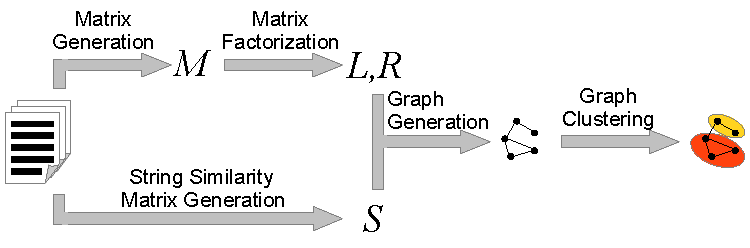
\includegraphics[width=0.9\textwidth]{chapter_three/unstructured_annotation/LD4IE_ISWC_CDCR/cdcr_SystemOverview.pdf}
\caption{The five steps of our approach.}
\label{fig:SystemOverview}
\end{figure}

%\todo[inline]{all: If somebody knows a program with which I can create a better picture than this, please let me know. Axel: Picture is fine}
%\todo[inline]{Micha: Refactor this section. Axel: Done}

\subsection{Matrix Generation}
%\todo[inline]{Micha}
The first step of our approach consists of generating a matrix which describes the context of every named entity mention inside the texts by means of a bag of words.
To this end, the given corpus is preprocessed by tokenizing the documents, removing stop words and indexing the remaining tokens.
In these tokenized documents, the context of a named entity mention is defined as the multiset of tokens inside a window with the size $\pm \sigma$ that is centered on the named entity's tokens.
The contexts are stored in a matrix $M$ containing a row for every named entity mention and a column for every indexed word.
The entries of the matrix are the counts of the words inside the entity mention's context.
As an example, let us consider the sentence 
\begin{ex}
\texttt{Yesterday, VW's CEO presented the new \underline{Golf} in Munich}.
\end{ex}
from which the stopwords \{\texttt{the}, \texttt{in}\} are removed.
For the window size $\sigma = 1$, we get the bag-of-word multiset \{\texttt{new} (1), \texttt{Munich} (1)\} as representation of ``Golf''.
Within the vector space spawned by (\texttt{presented}, \texttt{new}, \texttt{Munich}, \texttt{Germany}), this mention has the vector representation $(0, 1, 1, 0)$.
In the following, we will consider five entity mentions $g_1$, $g_2$, $g_3$, $g_4$ and $g_5$ labelled with the same word ``golf'' as example. 
These entity mentions will be assumed to be represented by the vectors 
$g_1 = (2,2,2,0)$, $g_2 = (1, 0, 0, 1)$, $g_3= (0,0,0,1)$, $g_4=(1, 0, 0, 0)$ and $g_5=(0, 1,1,0)$. 

\subsection{Matrix Factorization}
The matrix $M$ is now a matrix of dimensions $n \times m$ (denoted $M(n,m)$). 
The goal of a matrix factorization is to compute the matrices $L(n, \rho)$ and $R(m, \rho)$ such that $M \approx LR^{\top}$.
We call $\rho \in \mathbb{N} \backslash {0}$ the \emph{rank} of the factorization.
Several approaches have been used to factorize matrices.
Here, we loosely follow the tensor factorization approach presented in~\cite{DBLP:conf/www/NickelTK12}: Given two matrices $L$ and $R$ that are supposed to be the factors of $M$, the overall quadratic error of the approximation is the square Frobenius norm of $E = M - RL^{\top}$, i.e., $||E||_F^2 = ||M - RL^{\top}||_F^2$.
%We can express each entry of the squared Frobenius norm as follows:
%\begin{equation}
%e_{ij}^2 = \left(m_{ij} - \sum\limits_{k = 1}^r r_{ik}l_{jk}\right)^2.
%\end{equation}
%The error is minimal when the first partial derivative of $e_{ij}^2$ becomes 0.
%Thus, we need to minimize the values
%\begin{equation}
%\frac{\partial e_{ij}}{\partial r_{ik}} = -2 e_{ij}l_{jk} 
%\end{equation}
%and
%\begin{equation}
%\frac{\partial e_{ij}}{\partial l_{jk}} = -2 e_{ij}r_{ik}.
%\end{equation}
Previous works have shown that to prevent overfitting, the error function to minimize must be extended.
While several approaches have been suggested to this end, we adopt the error expression given by $||E||_F^2 - \frac{\lambda}{2}(||R||_F^2 + ||L||_F^2)$, where $\lambda \in [0, 1]$ controls how well $L$ and $R$ fit $M$. 
Thus, the error derivatives are as follows:
\begin{equation}
\frac{\partial e_{ij}}{\partial r_{ik}} = -2 e_{ij}l_{jk} + \lambda r_{ik}  
\end{equation}
 and 
\begin{equation}
\frac{\partial e_{ij}}{\partial l_{jk}} = -2 e_{ij}r_{ik} + \lambda l_{jk}.  
\end{equation}
We can now adopt a gradient descent approach to update the matrices $L$ and $R$ and reduce the error they lead to by overwriting each $l_{ik}$ resp $r_{jk}$ as follows:
\begin{equation}
l_{jk} \leftarrow l_{jk} - \alpha \frac{\partial e_{ij}}{\partial l_{jk}} = l_{jk} + \alpha \left(2 \sum\limits_{i=1}^n e_{ij}r_{ik} - \lambda l_{jk} \right)
\end{equation}
and
\begin{equation}
r_{ik} \leftarrow r_{ik} - \alpha \frac{\partial e_{ij}}{\partial r_{ik}} = r_{ik} + \alpha \left(2 \sum\limits_{j=1}^j e_{ij}l_{jk} - \lambda r_{ik} \right).
\end{equation}
We initialize $L$ and $R$ with random entries between 0 and $\max m_{ij}$.
%One problem that has remained unaddressed so far are the initialization of $L$ and $R$ as well as determining the correct settings for the parameters $r$, $\alpha$ and $\lambda$.
For our example, we get
\begin{equation}
M = \left(
\begin{matrix}
 2 & 2 & 2 & 0 \\
 1 & 0 & 0 & 1 \\
 0 & 0 & 0 & 1 \\
 1 & 0 & 0 & 0 \\
 0 & 1 & 1 & 0
\end{matrix} \right).
\end{equation}
For $\rho=2$, our approach computes
\begin{equation}
L = \left(
\begin{matrix}
  1.385 & 1.102 \\
 -0.006 & 0.501  \\
  0.079 & -0.051  \\
 -0.234 & 0.712 \\
  0.933 & -0.168
\end{matrix} \right)
\quad \text{and} \quad R = \left(
\begin{matrix}
 0.331 & 1.406 \\
 1.059 & 0.446 \\
 1.118 & 0.363 \\
 0.062 & 0.066
\end{matrix} \right).
\end{equation}
The intuition behind our approach is that $L$ is a better and compressed description of the entity mentions than $M$.
Hence, we now use $L$ in combination with a string similarity function to compute the similarity of entity mentions.

\subsection{String Similarity Matrix}
The string similarity matrix $S$ is an optional feature of our approach.
Each entry $s_{ij}$ of $S$ describes the similarity between the label of the $i$th and the $j$th entity in our input corpus.
Assuming a symmetric string similarity function such as the 3-gram similarity (which we use in our experiments), 
we also get a symmetric string similarity matrix $S$.
%Compute string similarity matrix $S$ using $n$-gram similarity with $n=3$.
We assume $s_{ij} = 1$ if no string similarity is specified.
$s_{ij} = 1$ also holds for our example, as all mentions are labelled with ``golf''.

\subsection{Graph Generation}
The aim of the graph generation is to generate a similarity graph $G = (V, E, w)$ that will allow detecting mentions of the same real-world object through clustering.
The set of vertices of $V$ is the set of entity mentions in our corpus.
We define the weight function $w: V \times V \rightarrow [0, 1]$ as $w(v_i, v_j) = s_{ij} \times \frac{l_{(i,\cdot)} \cdot l_{(j,\cdot)}}{||l_{(i,\cdot)}|| \times ||l_{(j,\cdot)}||}$, where $l_{(i,\cdot)}$ is the $i$th row-vector of $L$ and stands for the latent description of the $i$th entity mention in the corpus.
Given that many graph clustering approaches are polynomial in the number of edges, we can control $|E|$ by only setting an edge between $v_i$ and $v_j$ if $w(v_i, v_j) \geq \theta \in [0, 1]$.
%Remove edges with $g_{ij} \le \theta$ (=threshold)
For $\theta = 0.3$ and $\rho=2$ we end up with the graph displayed in Figure~\ref{fig:latent}. 
As comparison, Figure~\ref{fig:original} shows the graph obtained with by setting $L = M$, i.e., generating $G$ without using latent features.

\begin{figure}
\centering
\usetikzlibrary{arrows}

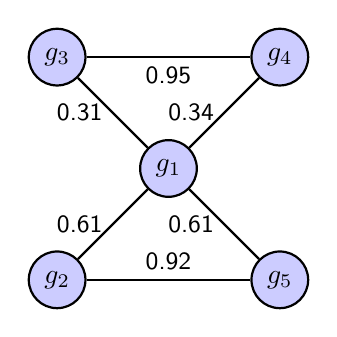
\begin{tikzpicture}[auto,node distance=2cm,
  thick,main node/.style={circle,fill=blue!20,draw,font=\sffamily\bfseries}]

  \node[main node] (1) {$g_1$};
  \node[main node] (2) [below left of=1] {$g_2$};
  \node[main node] (3) [above left of=1] {$g_3$};
  \node[main node] (4) [above right of=1] {$g_4$};
  \node[main node] (5) [below right of=1] {$g_5$};

  \path[every node/.style={font=\sffamily\small}]
    (1) edge node [left] {0.61} (2)
        edge node [left] {0.31} (3)
        edge node [left] {0.34} (4)
        edge node [left] {0.61} (5)
    (3) edge node [below] {0.95} (4)
    (2) edge node [above] {0.92} (5);    
\end{tikzpicture}
\caption{Graph generated using $\rho=2$}
\label{fig:latent}
\end{figure}

\begin{figure}
\centering
\usetikzlibrary{arrows}
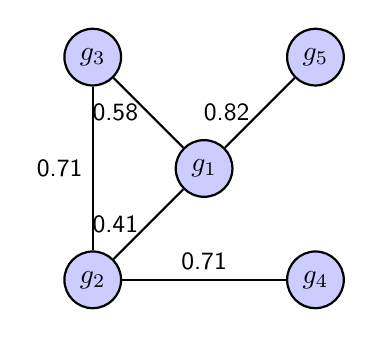
\begin{tikzpicture}[auto,node distance=2cm,
  thick,main node/.style={circle,fill=blue!20,draw,font=\sffamily\bfseries}]

  \node[main node] (1) {$g_1$};
  \node[main node] (2) [below left of=1] {$g_2$};
  \node[main node] (3) [above left of=1] {$g_3$};
  \node[main node] (4) [below right of=1] {$g_4$};
  \node[main node] (5) [above right of=1] {$g_5$};

  \path[every node/.style={font=\sffamily\small}]
    (1) edge node [left] {0.41} (2)
        edge node [left] {0.58} (3)
        edge node [left] {0.82} (5)
    (2) edge node [left] {0.71} (3)
    (2) edge node [above] {0.71} (4);    
\end{tikzpicture}
\caption{Graph generated using $M$ instead of $L$}
\label{fig:original}
\end{figure}

\subsection{Graph Clustering}
%\todo[inline]{Axel}
We now cluster the graph $G$ to detect mentions that stand for the same real-world object.
Our approach can rely on any graph clustering approach.
In our current implementation, we rely on the BorderFlow algorithm~\cite{DBLP:conf/cicling/NgomoS09} because it is parameter-free.
BorderFlow regards any set $C \subseteq V$ as having a \emph{border} $b(C) = \{v \in C: \exists u \in V \backslash C \mbox{ with } (v, u) \in E\}$.
The \emph{flow} $\Omega(C_1, C_2)$ between two sets $C_1 \subseteq V$ and  $C_2 \subseteq V$ is defined as $\Omega(C_1, C_2) = \sum\limits_{v \in C_1, u \in C_2} w(v, u)$.
Based on these definitions, BorderFlow implements a local graph clustering paradigm by mapping each node $v \in V$ to the set of nodes $C \subseteq V$ that is such that $v \in C$ and $C$ is a node-maximal set w.r.t. the function 
\begin{equation}
bf(C) = \frac{\Omega(b(C), C)}{\Omega(b(C), V \backslash C)}.
\end{equation}
While finding the optimal $C$ for each $v$ can be very time-consuming, the heuristic presented in~\cite{DBLP:bibsonomy_NGO10b} allows determining an approximation of $C$ in an efficient manner.
We employ this heuristic herein.

Now, the result of BorderFlow is not a partitioning of the graph.
Rather, clusters may overlap.
We thus employ a \emph{hardening} approach to generate a partitioning of the input graph.
To this end, each node $v\in V$ which belongs to two different clusters $C_1$ and $C_2$ is assigned to $C_1$ iff
\begin{equation}
bf(C_1 \cup \{v\}) + bf(C_2 \backslash \{v\}) \geq bf(C_2 \cup \{v\}) + bf(C_1 \backslash \{v\}).
\end{equation}
In all other cases, $v$ is assigned to $C_2$.
We call this form of hardening \emph{flow maximization}.
Other forms of hardening can be conceived of, e.g., minimizing the number of unions operations that need to be carried out to achieve a partitioning of the graph (\emph{set-based}).

For our example, we get the clusters $\{g_1, g_5\}$ and $\{g_2, g_3, g_4\}$ for $\rho=2$ when using BorderFlow with any partitioning approach.
If we replace $L$ with $M$, we get the clusters  $\{g_1\}$, $\{g_2, g_4\}$ and $\{g_3, g_5\}$.
This result on toy data already suggests that matrix factorization leads to results that differ from those gathered when using raw data.
In the subsequent section, we show empirically that using $L$ to generate $G$ leads to more accurate results than using $M$ to generate $G$.

\section{Evaluation}

\label{cha314:sec:evalval}

\subsection{Experimental Setup}

\subsubsection{Goals}
The goal of our experiments was two-fold. First, we wanted to measure the effect of the different parameters on our approach.
Moreover, we wanted to know whether the factorization outperforms a comparable baseline.
To achieve the first goal of our experiments, we conducted experiments where we varied the rank $\rho$ as well as the window size $\sigma$ while keeping all other parameters fixed.
We addressed the second goal by creating a baseline as follows: We ran our pipeline as described in the sections above with the sole difference that (1) we did not carry out a factorization and (2) we use $M$ instead of $L$ as input for the graph clustering. All other steps (matrix generation, graph generation, graph clustering) remained unchanged.
The similarity threshold for the graph generation is set to $\theta=0.1$ for all our experiments.

\subsubsection{Datasets}
We use the three corpora of the $\mbox{N}^3$ collection~\cite{n3} in our experiments.
%\todo[inline]{Actually here could be an error, which leads to very high f-measure}
%Each corpus was annotated manually, i.e., each entity mention was mapped to an URI from DBpedia~\cite{lehmann2014dbpedia} or a URI from the \url{http://aksw.org/} namespace if no corresponding resource could be found in DBpedia.
%
\begin{itemize}
\item The \textbf{News-100} corpus comprises 100 German news articles from \url{news.de}.
Each of these articles contains the German word ``Golf''---a homonym that has three different meanings inside these documents.
The word could mean (a) a gulf, e.g., the Mexican gulf, (b) the ball sport or (c) a compact car of the German manufacturer Volkswagen.
This is clearly the most difficult dataset, as many resources share exactly the same name but have different meanings. 
\item The \textbf{Reuters-128} corpus contains 128 English economy news articles from the Reuters news agency.
The documents in this dataset are smaller than the ones from the News-100 corpus providing a shallow context.
\item The third corpus, \textbf{RSS-500}, contains 500 documents each with only one sentence.
The sentences were randomly chosen from a larger amount of RSS news feeds, as described in~\cite{GER+13}.
Every sentence contains exactly two named entities.
\end{itemize}
Table~\ref{tab:corpusStats} provides further detailed information about the corpora.
On average, each named entity occurs nearly 5 times in the News-100 corpus.
Within the Reuters-128 corpus nearly two mentions per named entity exist on average while in the RSS-500 corpus only every tenth entity is mentioned more than once.

%\todo[inline]{Micha: describe N${}^{3}$}

\begin{table}[thb]
    \caption{Features of the corpora}
    \begin{tabular}{lp{0.7cm}rp{0.3cm}p{0.7cm}rp{0.2cm}p{0.6cm}rp{0.3cm}}
    \toprule
     & \multicolumn{3}{c}{\textbf{News-100}} & \multicolumn{3}{c}{\textbf{Reuters-128}} & \multicolumn{3}{c}{\textbf{RSS-500}} \\
    \midrule
    Documents && 100 &&& 128 &&& 500 &\\
	Tokens && 48199 &&& 33413 &&& 31640 &\\
	Entities && 362 &&& 444 &&& 849 &\\
    Mentions && 1655 &&& 880 &&& 1000 &\\
	\bottomrule
	\end{tabular}
	\centering
	\label{tab:corpusStats}
\end{table}

\subsection{Results}

\subsubsection{Influence of rank}
In our first series of experiments, we fixed the window size to 4 and measured the influence of the rank $\rho$ on the precision, recall and F-measure. 
The left side of Figure~\ref{fig:results} shows the results of our experiments on the three datasets.
Most importantly, our results show that we outperform the baseline in most settings.
We achieve the best increase of performance on the RSS-500 corpus, where we achieve a 20.5\% increase in F-measure over the baseline.
This result suggest that our approach does not tend to overgeneralize through the compression on information that is carried out during the factorization.
Instead, our results suggest that we get rid of a significant amount of noise while factorizing.
Our results on the other two datasets show that we also achieve a better F-measure (increases of 18.2\% on Reuters-128 and 6.3\% on News-100, see Table~\ref{tab:improvements}). 
An analysis of the results reveals that this increase is mostly due to the significant increase in precision that we achieve in most settings.
On the other hand, our recall is rarely ever worse than that of the baseline.
This suggests that BorderFlow tends to generate smaller clusters with factorization than when the baseline approach is used.
We measure the statistical significance of our results using a Wilcoxon signed rank-test with 95\% confidence.
Our results are significant in all cases.%\todo[inline]{Check this}

\subsubsection{Influence of window size}
In this experiment, we set the rank to 100 for all experiments and measured the effect of the window size on the overall F-measure of our approach.
The right half of Figure~\ref{fig:results} shows the results of this series of experiments on the three datasets.
Overall, our results suggest that for this rank, the window size does not have a major influence on the F-measure. 
This also seems to hold for other ranks.
Interestingly, a small window size seems to lead to good results in most cases when we use the factorization. While we assume that this might be due to the factorization being able to convert the two words within the window to their latent features    
This result indicates that small window sizes suffice for our approach to achieve better F-measures than the baseline on the CDCR problem.
This might mean that a small set of words is already sufficient to disambiguate resources across different documents.

\begin{figure}[t!]
\centering
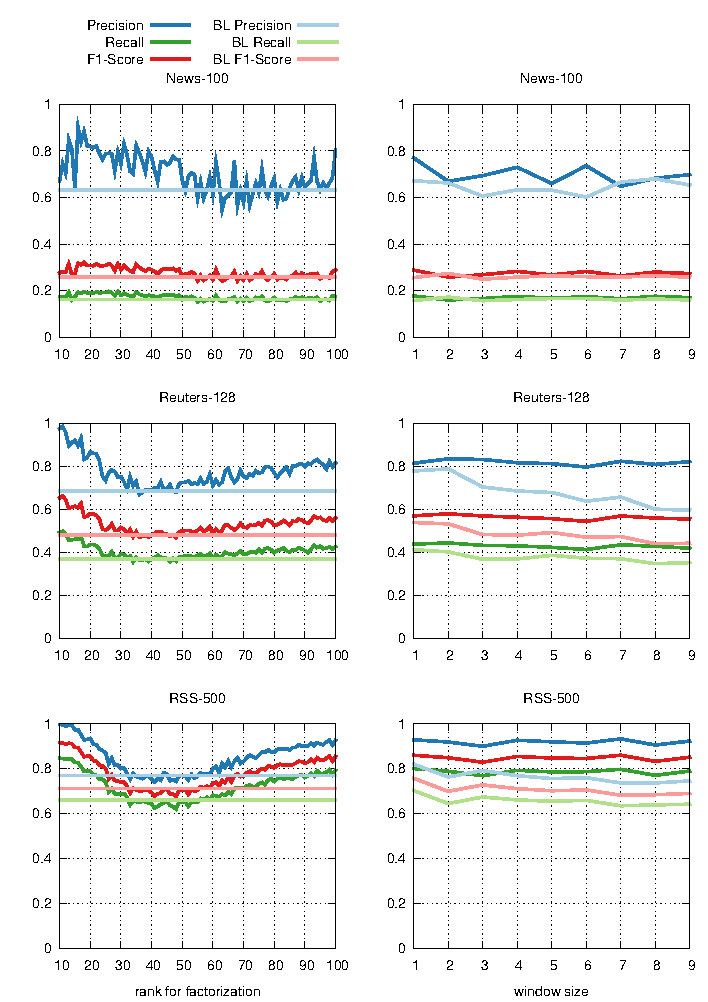
\includegraphics[width = \textwidth]{chapter_three/unstructured_annotation/LD4IE_ISWC_CDCR/cdcr_results_Flow.pdf}
\caption{Precision, recall and F1-score of our approach with different ranks (left) and different window sizes (right) compared to the baseline (BL). The diagrams show the results for the flow maximization hardening.}
\label{fig:results}
\end{figure}
\afterpage{\clearpage}

\subsection{Effect of hardening}
In all results presented above, we used a hardening based on the borderflow ratio.
We also implemented the set-based hardening mentioned above and compared the results we achieve with this hardening.
Overall, our results suggest that the borderflow-maximization approach that we used for hardening generates the best results both for the baseline and our approach. 
Moreover, we outperform the baseline independently from the hardening used.

\begin{table}[htb]
    \caption{Best improvements in F-measure of our approach (OA) over the baseline (BL)}
    \begin{tabular}{lp{1cm}p{0.25cm}rp{1cm}p{0.25cm}rp{1cm}p{0.25cm}rp{1cm}p{0.25cm}r}
    \toprule
     && \multicolumn{5}{c}{\textbf{Flow Maximization}} && \multicolumn{5}{c}{\textbf{Set-Based}} \\
     && \multicolumn{2}{c}{BL} && \multicolumn{2}{c}{OA} && \multicolumn{2}{c}{BL} && \multicolumn{2}{c}{OA} \\
    \midrule
    News-100        &&& 25.86  &&& \textbf{32.21} &&& 23.87  &&& \textbf{28.81} \\
	Reuters-128     &&& 47.89  &&& \textbf{66.16} &&& 47.00  &&& \textbf{56.65} \\
	RSS-500         &&& 71.11  &&& \textbf{91.62} &&& 69.57  &&& \textbf{85.71} \\
	\bottomrule
	\end{tabular}
	\centering
	\label{tab:improvements}
\end{table}

%\subsection{Scalability}\todo[inline]{Please fill gaps}
%One last question that we addressed is the scalability of our approach.
%We ran our experiments on a Debian machine (Intel Xeon 3.10GHz, 8GB RAM).
%On average, the baseline experiments ran 22.7s for News-100, ??? for Reuters-128 and ??? for RSS-500.
%In contrast, the experiments with factorization ran ??? for News-100, ??? for Reuters-128 and ??? for RSS-500.
%These results suggest that our approach scales when and does not produce a significant overhead in runtime while generating significantly better results.

\subsubsection{Discussion}
Overall, our initial results suggest that we indeed outperform the proposed baseline by using matrix factorization (see Table~\ref{tab:improvements}).
Still, many questions do remain open.
The most important question that we did not address is when should a high rank be used?
First, in our experiments, $\rho=10$ was sufficient across all datasets to outperform the baseline. 
To the best of our knowledge, finding the optimal rank for a factorization problem is an open question.
Nevertheless, we think that the answer to this question lies in the amount of information contained in the corpus.
The higher the information density of a corpus, the higher the rank required to characterize entity adequately.
A second question that remains unanswered is whether we can improve the results of the factorization by considering known resources in the dataset.
We will address this question in future work by disambiguating using a combination of textual information and Linked Data.
%\todo[inline]{Micha: Refactor the current figure. It doesn't look really nice.}

%\subsubsection{Runtime}
%We also measured the runtime of our approach across all experiments. Our results suggest that our approach can actually lead to significantly smaller runtimes. However, the settings in which we achieve the best runtimes correspond to settings in which the overall runtime of our approach is comparable to that of the baseline. This is obviously a satisfactory results as it means that we can achieve better F-measure without requiring significantly higher processing times.

\section{Conclusion}
\label{cha314:sec:conclusion}
In this paper, we presented a CDCR approach based on latent features.
We showed that our approach can outperform our baseline by more than 10\% F-measure.
%Moreover, we showed that our approach scales well and can thus be used on large datasets.
We will use our approach to complement the entity linking framework~\cite{agdistis_iswc} when it is used in batch mode, i.e., over a document corpus at once.
Moreover, we will develop means to detect an appropriate rank for factorization.
To this end, we plan to use the derivative of the mean squared error $||M - LR^{\top}||^2_F$.
Finally, we will develop a deterministic approach to initialize $L$ and $R$. 
Preliminary results on random matrices show that we can already reduce the initial value of $||E||^2_F$ by more approximately 40\%, leading to a significantly faster convergence of the factorization.



%\end{document}


\begin{comment}
\begin{table}[htb]
    \caption{Best improvements of our approach over the baseline}
    \begin{tabular}{lp{0.5cm}cp{0.5cm}cp{0.5cm}c}
    \toprule
     && \multicolumn{1}{c}{\textbf{Rank}} && \multicolumn{1}{c}{\textbf{Baseline (F1)}} && \multicolumn{1}{c}{\textbf{Our approach (F1)}} \\
    \midrule
    News-100        && 11   && 56.78  && 62.99 \\
	Reuters-128     && 91   && 68.23  && 71.63 \\
	RSS-500         && 97   && 79.31  && 88.40 \\
	\bottomrule
	\end{tabular}
	\centering
	\label{tab:improvements}
\end{table}
\end{comment}

\begin{comment}
\subsection{Initialization of $L$ and $R$}
In most approaches, the matrices $L$ and $R$ are initialized by using random values.
While this approach still leads to converging results in practical applications, it is unsatisfactory as the results of the factorization may be different across different initializations.
We address the initialization problem by using a correlation-based approach.
The intuition behind our approach is that the latent features describe a space whose basic vectors stand for weakly correlated dimensions. 
We can thus initialize the matrices $L$ (and analogously the matrix $R$) by detecting the rows (resp. columns) that display the smallest correlation to other rows and using those as our initialization for $L$.
We go about implementing this intuition as follows: Let 
\begin{equation}
B = M \times M^\top \mbox{ and } A = \frac{B}{\max\limits_{i, j} b_{ij}}.
\end{equation}
The matrix $A$ encompasses how correlated the rows in $M$ are.
We assign each row $a_{i}$ a weight $w_i = \sum_{j=1}{n} a_{ij}$.
The weight $w_i$ tells us how correlated $a_i$ is to $a_1 \ldots a_n$.
We now sort the rows according to their weights in ascending order and select the r rows with the smallest weight.
These rows are then used to initialize $L$, ergo $l_1 = a_k$ with $\forall i \neq k, w_i \geq w_k$.  

The matrix $R$ can be initialized analogously by setting 
\begin{equation}
B = M^\top \times M \mbox{ and } A = \frac{B}{\max\limits_{i, j} b_{ij}}.
\end{equation}
\todo{Add example}

\begin{itemize}
\item use FOX to do NER over several documents \todo{No need for FOX in the experiments. Simply use the benchmarks directly.} 
\todo{Now it is implemented and getting back to the original work would be cumbersome.} 
\item describe an entity by its neighbors, i.e., window size and latent features
\item use cosine similarity as a baseline
\item cluster those entities across documents using Axels framework
\item named entities are the same resources if they end up in the same cluster...\todo[inline]{RU: I fear the noise hear when number of clusters is too low}
\item formulate good URIs for them, see http://www.w3.org/TR/cooluris/

\end{itemize}

LR^T = 

  5,103 1,896 -0,712 1,555
  3,412 1,274 -0,450 1,085
  1,540 1,040  1,780 3,949
  1,169 0,799  1,394 3,073
 -0,438 0,543  3,076 5,125
\end{comment}

